%versi 2 (8-10-2016) 
\chapter{Pendahuluan}
\label{chap:intro}
   
\section{Latar Belakang}
\label{sec:label}

Tugas merupakan suatu bentuk pembelajaran dan penilaian yang diberikan oleh pengajar kepada pelajar untuk membantu pelajar mendalami materi yang sudah diberikan. Pembagian tugas yang diberikan dapat dibagi menjadi 2 jenis yakni tugas individu dan tugas kelompok. Tugas individu merupakan tugas yang hanya ditanggung oleh satu individu sedangkan, tugas kelompok merupakan tugas yang ditanggung oleh beberapa individu. Tugas selanjutnya akan dikumpulkan kepada pengajar dan diberikan penilaian berdasarkan tingkat ketepatan jawaban dari tugas tersebut. Pengumpulan dan pengecekan tugas terutama \textit{coding} secara manual memiliki kekurangan dimana diperlukan banyak langkah dalam melakukan pengecekan dan pengiriman nilai. Pengecekan secara manual juga terdapat kesulitan dalam pengecekan yakni, kekurangan dalam pengecekan plagiat antara tugas pelajar. Maka, dibutuhkan perangkat lunak untuk melakukan pengecekan secara otomatis salah satunya adalah \textit{Online Judge}.

\textit{Online Judge} merupakan sebuah perangkat lunak berbasis web yang dapat melakukan pengecekan \textit{program} sesuai dengan standar yang sudah diberikan. Perangkat lunak ini dapat menerima jawaban dari pelajar dan melakukan pengecekan secara otomatis dan memberikan keluaran berupa nilai dari pelajar tersebut. Salah satu perangkat lunak \textit{Online Judge} terdapat pada Informatika Unpar bernama SharIF Judge (dapat dilihat pada Gambar  \ref{fig:judgeawal}). 

\begin{figure}[H]
	\centering  
	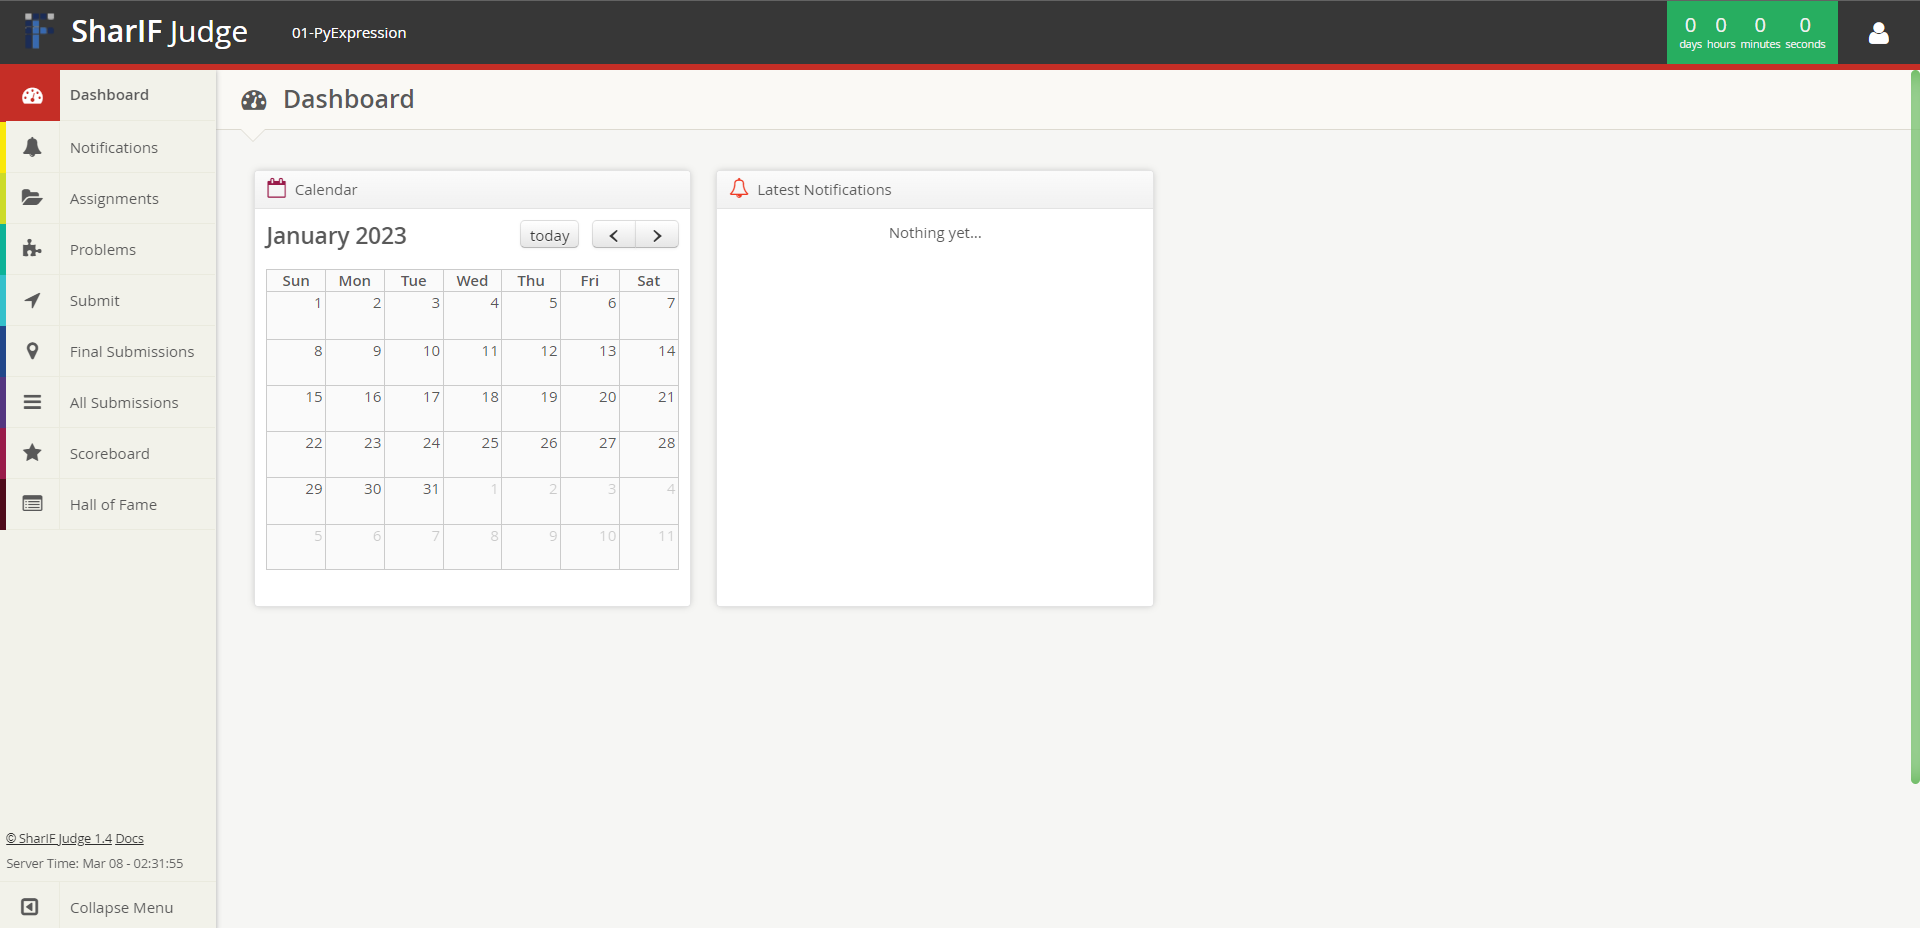
\includegraphics[scale=0.3]{judgeawal}  
	\caption[Tampilan halaman \textit{SharIF Judge}]{Tampilan halaman \textit{SharIF Judge}} 
	\label{fig:judgeawal} 
\end{figure} 


SharIF Judge merupakan sebuah alat \textit{open source} untuk menilai kode dengan beberapa bahasa seperti C, C++, Java, dan Python secara online. SharIF Judge dibentuk menggunakan \textit{framework} CodeIgniter 3 yang merupakan \textit{framework} berbasis PHP dan dimodifikasi sesuai dengan kebutuhan Informatika Unpar untuk mengumpulkan tugas dan ujian mahasiswa. 

CodeIgniter 3 merupakan sebuah \textit{framework} gratis yang bertujuan untuk mempermudah dalam membentuk sebuah aplikasi \textit{website} menggunakan PHP. CodeIgniter 3 menggunakan struktur MVC yang membagi file menjadi 3 buah yaitu Model, View, Controller. Selain itu, CodeIgniter 3 merupakan \textit{framework} ringan dan menyediakan banyak \textit{library} untuk digunakan oleh penggunanya. 

CodeIgniter 3 sudah memasuki fase \textit{maintenance} sehingga tidak akan mendapatkan \textit{update} lebih lanjut dari pembentuknya. CodeIgniter 3 pada akhirnya akan tidak dapat dipakai dan akan hilangnya dokumentasi dari situs web resmi. Sehingga, perangkat lunak yang menggunakan CodeIgniter 3 perlu dikonversi ke \textit{framework} CodeIgniter dengan versi terbaru yakni CodeIgniter 4.

CodeIgniter 4 merupakan versi terbaru dari \textit{framework} CodeIgniter yang memiliki banyak perubahan fitur dari versi sebelumnya. CodeIgniter 4 dibentuk menggunakan versi PHP 7.4 sedangkan CodeIgniter 3 dibentuk menggunakan versi PHP 5.6. CodeIgniter 4 membagi file menggunakan struktur MVC namun, memiliki struktrur folder berbeda dengan versi sebelumnya.

Pada skripsi ini, akan dilakukan konversi SharIF Judge dari CodeIgniter 3 menjadi CodeIgniter 4. Konversi dilakukan karena CodeIgniter 3 sudah memasukin fase \textit{maintenance} sehingga CodeIgniter 3 hanya akan mendapatkan \textit{security update}.

\section{Rumusan Masalah}
\label{sec:rumusan}
\begin{itemize}
\item Apa standar yang ada sehingga CodeIgniter 3 perlu dikoversi CodeIgniter 4?
	\item Bagaimana cara melakukan konversi CodeIgniter 3 menjadi CodeIgniter 4?
	\item Bagaimana mengevaluasi kode SharIF Judge dan mengubahnya agar dapat berjalan di CodeIgniter 4?
\end{itemize}
\section{Tujuan}
\label{sec:tujuan}
\begin{itemize}
	\item Mencari standar yang dibutuhkan sehingga CodeIgniter 3 perlu di konversi mendjadi CodeIgniter 4.
	\item Melakukan konversi dengan megubah kode sesuai dengan CodeIgniter 4.
	\item Melakukan evaluasi kode SharIF Judge dan mengubahnya agar dapat berjalan di CodeIgniter 4.
\end{itemize}

\section{Batasan Masalah}
\label{sec:batasan}
Perangkat lunak hanya akan dikonversi sesuai dengan perangkat lunak yang sudah dibentuk. Kesalahan-kesalahan lain (tidak dapat di run pada windows,) akan ditulis di keluaran perangkat lunak apa adanya.

\section{Metodologi}
\label{sec:metlit}
Metodologi yang dilakukan dalam melakukan penelitian ini adalah sebagian berikut:
\begin{enumerate}
	\item Melakukan analisis dan eksplorasi fungsi-fungsi perangkat lunak SharIF Judge.
	\item Melakukan analisis 
	\item Melakukan konversi perangkat lunak dari CodeIgniter 3 menjadi CodeIgniter 4.
	\item Melakukan pengujian dan eksperimen terhadap perangkat lunak yang sudah di konversi.
	\item Menyelesaikan pembentukan dokumen
\end{enumerate}

\section{Sistematika Pembahasan}
\label{sec:sispem}
Penelitian ini akan dibahas dalam enam bab yang masing-masing berisi:
\begin{enumerate}
	\item \textbf{Bab 1:} Pendahuluan
	Bab ini berisi latar belakang, rumusan masalah,tujuan, batasan masalah, metodologi, dan sistematika pembahasan.
	\item \textbf{Bab 2:} Dasar Teori
	Bab ini berisi 
	\item \textbf{Bab 3:} Analisis
	\item \textbf{Bab 4:} Perancangan
	\item \textbf{Bab 5:} Implementasi dan Pengujian
	\item \textbf{Bab 6:} Kesimpulan dan Saran
\end{enumerate}
